\documentclass[11pt, titlepage]{article}
\usepackage{amsmath,amsthm,amssymb}
\usepackage{hyperref, pgf, tikz}
\usepackage{fancyhdr}
\usetikzlibrary{arrows}
\usepackage[margin=1.25in]{geometry}
\usepackage{graphicx}                     
\pagestyle{fancy}
\usepackage{array}
%\usepackage{wrapfig}

\lhead{Lab \#2}
\rhead{\thepage}
\cfoot{}

\title{Projectile Motion: The Ballistic Pendulum \\ \ \\ \large Lab \#2}
\author{Name: Avery Karlin \\ Partner: Alon Levin}
\date{}
\begin{document}

\maketitle

\begin{center}
\LARGE Projectile Motion: The Ballistic Penudulum
\end{center}

\section*{Objective}
The objective of the lab is to measure the initial velocity of a projectile, both through a ballistic pendulum and through range distance measurements, and to measure the optimal projectile firing angle for maximum distance. 
\section*{Introduction}
The ballistic pendulum is an object which fires a metal ball from a spring gun, catched by a specific notch, which can then be used by conservation of momentum and mechanical energy to determine the initial velocity. Since all external forces are vertical, horizontal momentum is conserved during the collision, such that $$v_{x_o} = \frac{(m + M)V}{m}$$, where V is the velocity directly after the collision. By conservation of energy, ignoring rotational kinetic energy and loss of energy from friction and drag, kinetic directly after the collision is equal to the ending potential energy. Thus, $$\frac{1}{2}(m + M)V^2 = (m + M)gh$$, where V is the velocity directly after the collision once again. Thus, we can use these two equations to find $v_{x_o}$, without requiring V (after-collision). As a result, we get $$v_o = v_{x_o} = \frac{(M+m)\sqrt{2gh}}{m}$$.

Once we remove the pendulum, it functions as a horizontally-launched projectile, such that by the equations $x = v_{x_o}t$ and $y = frac{1}{2}gt^2$, such that $$v_o = v_{x_o} = \sqrt(\frac{gx^2}{2y}).$$ If we prop up the ballistic pendulum spring gun, it can function as a regular projectile, such that $x = v_{x_o}t$ and $0 = v_{y_o}t + \frac{1}{2}gt^2$, where $v_{y_o} = v_osin(\theta)$ and $v_{x_o} = v_ocos(\theta)$. Thus, we can solve for x, such that $$x = \frac{2v_o^2sin(\theta)cos(\theta)}{g},$$ giving us a formula for v_o, $$v_o = \sqrt{\frac{gx}{2sin(\theta)cos(\theta)}}.$$

\section*{Procedures and Results}

First, we set up the ballistic pendulum, placing the ball at the end of the gun, shooting it into the pendulum bob and allowing contact forces with the notches to slow it down, measuring the notch it ends at. We then measured the height of the pendulum bob from the surface, the mass of the ball, and the mass of the pendulum, all of which can be used to calculate the initial velocity.

Next, we remove the pendulum bob, so that there is no collision with the ball and the apparatus, we place it at some level above the ground and measure the distance from the gun by placing paper where it hits to indent the paper and allow the exact location to be measured, after which we fire the gun. Then, we measure the height of the gun to begin with, by which the initial velocity can be calculated.

Finally, we raise the spring gun to a desired angle, and fire, measuring the range of the projectile, using the angle to determine the initial velocity through the angle and range. 

\begin{figure}[p]
\centering
\hspace*{-8cm}
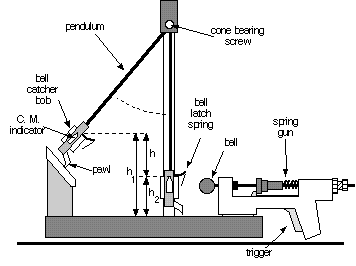
\includegraphics[scale=2]{lab2.jpg}
\vspace*{1cm}
\end{figure}

\begin{center}
$$\text{Height of} h_2 \text{of pointer with pendulum catch in closest-to-average notch number} = 0.094 m$$
$$\text{Height of} h_1 \text{of pointer with pendulum freely suspended} = 0.056 m$$
$$h = h_2 - h_1 = 0.038 m$$
$$\text{Mass of ball m} = 0.0691 kg$$
$$\text{Mass of pendulum M (bob and support)} = 0.28 kg$$
\begin{tabular}
{|m{17em}|m{17em}|}
\hline
Trials & Notch Number of Pendulum Catch \\
\hline
1 & 12\\
\hline
2 & 15\\
\hline
3 & 19\\
\hline
4 & 19\\
\hline
5 & 23\\
\hline
Average & 17.6\\
\hline
\end{tabular}

$$\text{Vertical distance of fall, y} = 0.5 m$$
$$v_{x_o} \text{(calculated)} = $$
$$\text{Percent difference between results of part A and B} = $$
\begin{tabular}
{|m{17em}|m{17em}|}
\hline
Trials & Range\\
\hline
1 & 2.2\\
\hline
2 & 2.155\\
\hline
3 & 2.105\\
\hline
4 & 2.123\\
\hline
5 & 2.125\\
\hline
Average & 2.1416\\
\hline
\end{tabular}

\begin{tabular}
{|m{17em}|m{17em}|}
\hline
Angle of projection & Average range \\
\hline
$20^o$ & 3.23\\
\hline
$30^o$ & 3.82\\
\hline
$40^o$ & 4.08\\
\hline
$45^o$ & 4.31\\
\hline
$50^o$ & 4.12\\
\hline
$60^o$ & 3.64\\
\hline
$70^o$ & 3.44\\
\hline
\end{tabular}
\end{center}

\section*{Discussion}
Sample calculations for the non-measured data are as shown:

$$v_o \text{ Ballistic Pendulum} = \frac{(M+m)\sqrt{2gh}}{m} = \frac{(0.0691 + 0.28)\sqrt{2*9.8*0.038}}{0.0691} = 4.36 m/s$$
$$v_o \text{ Horizontal Projectile} = \sqrt{\frac{gx^2}{2y}} = \sqrt{\frac{9.8*2.1416^2}{2*0.5}} = 6.704 m/s$$
$$\text{Ballistic Pendulum-Horizontal Projectile Percent Difference} = \frac{|v_{horiz} - v_{ball}|}{v_{horiz}} * 100\% = 35\%$$ 

\begin{figure}[p]
\centering
\hspace*{-16cm}
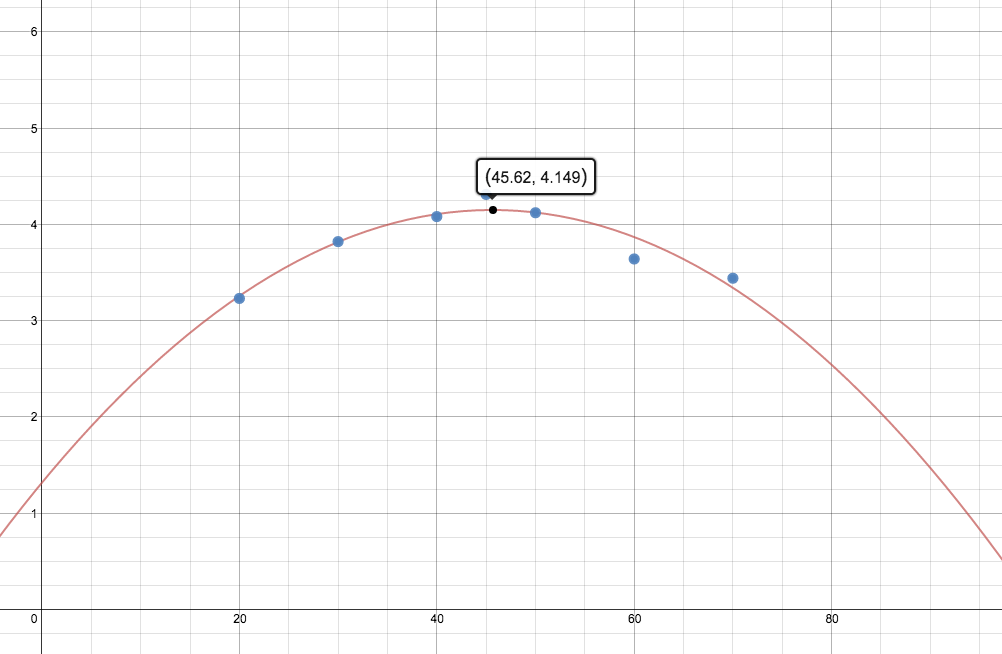
\includegraphics[scale=0.7, angle=0]{graph2.jpg}
\vspace*{-5cm}
\end{figure}

$$\text{Maximum Range Prediction} = 45.62^o$$
$$\text{Percent Difference} = 1.37\%$$

The large difference in the initial velocities calcuated by the ballistic pendulum and the horizontal projectile, other than being due to an error in either measurement, or a mechanical failure with the spring gun, could be attributed for the longer amount of time in the air for the horizontal projectile, allowing additional interference from drag. Drag would also explain the low amount of error in the final testing, due to the fact that the time spent in the air for all of the tests would be similar, unlike the ballistic pendulum, which would have little time spent airbourne.

\section*{Conclusion}
The initial velocity of the ballistic pendulum test was 4.36 m/s, while the initial velocity of the horizontal projectile test was 6.704 m/s, such that the percent difference is 35\%. The maximum range predicted by the projectile test is at $45.62^o$, with a percent difference of the actual ($45^o$) is 1.37\%.

\end{document}
